\documentclass[a4paper,ngerman]{article}

\usepackage[ngerman]{babel}
\usepackage[utf8]{inputenc}
\usepackage[
        pdftitle={Implementation eines Redis Client und Proxy für Protobuf und gRPC in C++},
        pdfauthor={Christoph Heiss}
]{hyperref}
\usepackage{fancyvrb}
\usepackage{parskip}
\usepackage{tabularx}

% Use minted for syntax highlighting.
\usepackage{minted}
% Some configuration for this document
\renewcommand{\listingscaption}{Codelisting}
\setminted{xleftmargin=20pt,linenos,frame=leftline,fontsize=\small,framesep=10pt,breaklines}

\usepackage{graphicx}
\usepackage[section]{placeins}
\usepackage{xcolor}
\hypersetup{
        colorlinks,
        linkcolor={violet!50!black},
        citecolor={blue!50!black},
        urlcolor={blue!80!black}
}

\graphicspath{{images/}}

\title{Implementation eines Redis Client und Proxy für Protobuf und gRPC in C++}
\author{Christoph Heiss}

\begin{document}

\begin{titlepage}
\maketitle
\thispagestyle{empty}
\end{titlepage}

\tableofcontents
\clearpage


%%%%%%%%%%%%%%%%%%%%%%%%%%%%%%%%%%%%%%%%%%%%%%%%%%%%%%%
%%%%%%%%%%%%%%%%%%%%%%%%%%%%%%%%%%%%%%%%%%%%%%%%%%%%%%%
\section{Lizenz}
\begin{Verbatim}[fontsize=\small]
Boost Software License - Version 1.0 - August 17th, 2003

Permission is hereby granted, free of charge, to any person or organization
obtaining a copy of the software and accompanying documentation covered by
this license (the "Software") to use, reproduce, display, distribute,
execute, and transmit the Software, and to prepare derivative works of the
Software, and to permit third-parties to whom the Software is furnished to
do so, all subject to the following:

The copyright notices in the Software and this entire statement, including
the above license grant, this restriction and the following disclaimer,
must be included in all copies of the Software, in whole or in part, and
all derivative works of the Software, unless such copies or derivative
works are solely in the form of machine-executable object code generated by
a source language processor.

THE SOFTWARE IS PROVIDED "AS IS", WITHOUT WARRANTY OF ANY KIND, EXPRESS OR
IMPLIED, INCLUDING BUT NOT LIMITED TO THE WARRANTIES OF MERCHANTABILITY,
FITNESS FOR A PARTICULAR PURPOSE, TITLE AND NON-INFRINGEMENT. IN NO EVENT
SHALL THE COPYRIGHT HOLDERS OR ANYONE DISTRIBUTING THE SOFTWARE BE LIABLE
FOR ANY DAMAGES OR OTHER LIABILITY, WHETHER IN CONTRACT, TORT OR OTHERWISE,
ARISING FROM, OUT OF OR IN CONNECTION WITH THE SOFTWARE OR THE USE OR OTHER
DEALINGS IN THE SOFTWARE.
\end{Verbatim}
\clearpage


%%%%%%%%%%%%%%%%%%%%%%%%%%%%%%%%%%%%%%%%%%%%%%%%%%%%%%%
%%%%%%%%%%%%%%%%%%%%%%%%%%%%%%%%%%%%%%%%%%%%%%%%%%%%%%%
\section{Redis}
\textbf{Redis}\footnote{\url{https://redis.io/}} ist eine sogenannte in-memory Datenbank. Diese Datenbanken zeichen sich hauptsächlich dadurch aus, das diese sämtliche Daten lediglich im Arbeitsspeicher ablegen, ohne diese auf ein permanentes Speichermedium zu schreiben. Dies ermöglicht eine hohe Performance, welche konventionelle Datenbanken nicht erreichen können, jedoch gehen diese Daten in Falle eines Absturzes verloren.

Der häufigste Anwendungszweck für diese Art von Datenbanken ist sie als Cache (Zwischenspeicher) für verteilte Anwendungen zu benutzen

\subsection{RESP}
Das \textbf{REdis Serialization Protocol} ist das Protokoll, das der Kommunikation zwischen Redis-Server und Clients zugrunde liegt. Die Designgrundlage für dieses Protokoll war ein Kompromiss aus Einfachheit, einfach zu verarbeiten und menschenlesbar.
Daraus entstand ein textbasiertes, prefix-basiertes Protokoll.

\textbf{libresply} implementiert den gesamten Protokoll-Umfang, inklusive \textit{Pipelining}\footnote{\url{https://redis.io/topics/pipelining}} und dem \textit{Redlock-Algorithmus}\footnote{\url{https://redis.io/topics/distlock}}.
Für normale Kommandos gibt ein einerseits ein rekursives, template-basiertes Serializierungsinterface als auch ein simpleres Interface zur Übergabe eines Arrays von Strings.

\textit{Pipelining} wird mittels eines eigenes Interfaces unterstützt. Der Vorteil von Pipelining ist die effiziertere und meist performantere Netzwerknutzung bei großen Datenmengen. Hierbei wird zunächst eine Reihe an Kommandos angesammelt und danach gemeinsam verschickt. Dieses Verfahren ermöglicht eine bessere Auslastung des Netzwerkes.

Der \textit{Redlock-Algorithmus} ist ein primitives Verfahren um eine Ressource zwischen verteilten Systemen zu synchronisieren.


%%%%%%%%%%%%%%%%%%%%%%%%%%%%%%%%%%%%%%%%%%%%%%%%%%%%%%%
%%%%%%%%%%%%%%%%%%%%%%%%%%%%%%%%%%%%%%%%%%%%%%%%%%%%%%%
\section{Architektur}
Die Architekur besteht im Wesentlichen aus der Library \textit{libresply} als Hauptbaustein sowie vier ausführbaren Programm und einer externen Komponente.

\begin{itemize}
        \item{\textbf{libresply}} implementiert das Protokoll \textit{RESP} zur Kommunikation mit einem Redis Server.
        \item{\textbf{redis-cli}} setzt auf libresply auf um ein einfaches Kommandozeilenwerkzeug zur Verwaltung von Redis Servern zu bilden.
        \item{\textbf{proxy}} bildetet eine Schnittstelle zwischen den Protobuf-basierten Protokoll und einem Redis Server.
        \item{\textbf{proto-cli}} implementiert ein einfaches Kommandozeilenwerkzeug zur Verwaltung von Redis Server unter Verwendung des Protobuf-basierten Protokolls und des Proxy-Servers.
        \item{\textbf{grpc-cli}} verfolgt den selben Ansatz wie \textit{proto-cli}, allerdings benutzt es zusätzlich zu Protobufs gRPC zur Kommunikation mit dem Proxy.
\end{itemize}

In Abb. \ref{img:structur} ist ein simples Umweltdiagramm des gesamten Projektes abgebildet. Auf diesem ist einfach und schnell zu sehen, wie die einzelnen Komponenten zusammenspielen.

\begin{figure}[H]
        \centering
        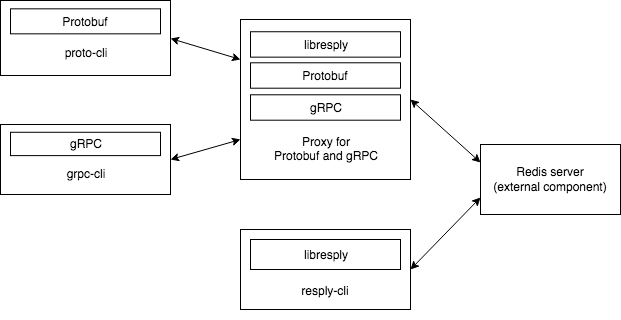
\includegraphics[width=1\linewidth]{umwelt}
        \caption{Umweltdiagramm des Projektes}
        \label{img:structur}
\end{figure}

\subsection{libresply}
\textbf{libresply} ist die Hauptkomponente dieses Projektes.
Für die Netzwerkkommunikation wird hierbei aus asio{\footnote{\url{http://think-async.com}} (die Standalone-Variante, ohne Boost) gesetzt und ist die einzige Drittanbieter-Library, die \textit{libresply} benötigt.

Sie besteht lediglich aus einem einzigen Header, \texttt{resply.h} der alles benötigte behinhaltet.
Dieses Dokument wird im Folgendenen auch zwei weitere, rein interne Klassen kurz beschreiben (siehe Tab. \ref{tab:libresply-classes}).

\begin{table}[H]
\centering
\begin{tabularx}{\linewidth}{|c|c|X|} \hline
        \textit{Name} & \textit{Sichtbarkeit} & \textit{Beschreibung} \\\hline
        Client & öffentlich & Implementiert die Hauptschnittstelle für die Nutzer der Library. \\\hline
        Pipeline & öffentlich & Implementiert ein ähnliches API wie \textit{Client}, basiert jedoch auf dem \textit{Pipelining} von Redis-Kommandos. \\\hline
        Result & öffentlich & Dient zur Speicherung von Weitergabe von Ergebnissen eines Redis-Kommandos. \\\hline
        RespParser & privat & Implementiert einen streambasierten Parser für Redis-Kommandos bzw. Antworten des Redis-Servers. \\\hline
        ClientImpl & privat & Implementiert sämtliche netzwerkbasierten Operationen von \textit{Client}. \\\hline
\end{tabularx}
\caption{Beschreibung aller Klassen von \textit{libresply}}
\label{tab:libresply-classes}
\end{table}


%%%%%%%%%%%%%%%%%%%%%%%%%%%%%%%%%%%%%%%%%%%%%%%%%%%%%%%
%%%%%%%%%%%%%%%%%%%%%%%%%%%%%%%%%%%%%%%%%%%%%%%%%%%%%%%
\section{Aufbau des Protobuf-basierenden Protokolls}
\label{sec:protobuf-message-structure}
\textbf{Protocol Buffers}\footnote{\url{https://developers.google.com/protocol-buffers}} ist ein Platform und Programmiersprachen unabhängiger Mechanismus, Daten binär und möglichst kompakt zu serializieren.

Der Aufbau einer Protobuf-Nachricht (\textit{message}) zwischen Proxy und \texttt{proto-cli} ist äußert simpel - ein Railroad Diagramm zur Beschreibung des Aufbau ist in Abb. \ref{img:railroad-protobuf-structure} zu sehen.

\begin{figure}[H]
        \centering
        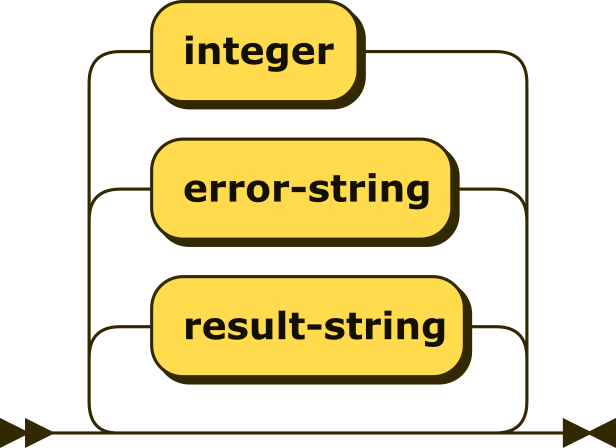
\includegraphics{protobuf}
        \caption{Railroad Diagramm des Aufbaus eines Protobuf-Kommandos.}
        \label{img:railroad-protobuf-structure}
\end{figure}

\subsection{Versand und Empfang von Nachrichten}
Zunächst wird eine 32-bit Zahl in Netzwerk-Byte-Reihenfolge (Big Endian)\footnote{\url{https://www.ibm.com/support/knowledgecenter/en/SSB27U_6.4.0/com.ibm.zvm.v640.kiml0/asonetw.htm}} gesendet. Diese repräsentiert die Größe der darauffolgenden Protobuf-Nachricht.
Im Falle das Clients enthält diese Nachricht zunächst die Kommando-Namen und danach sämtliche Argumente als Zeichenkette. Im Falle des Server bzw. Proxys enthält diese Nachricht die Antwort des Redis-Server, welche sowohl eine einfache Zahl, eine einfache Zeichenkette oder Fehlermeldung oder ein Array der vorhergehenden Datentypen.

%%%%%%%%%%%%%%%%%%%%%%%%%%%%%%%%%%%%%%%%%%%%%%%%%%%%%%%
%%%%%%%%%%%%%%%%%%%%%%%%%%%%%%%%%%%%%%%%%%%%%%%%%%%%%%%
\section{Aufbau des gRPC-basierenden Protokolls}
\textbf{gRPC}\footnote{\url{https://grpc.io}} ist ein von Google entwickeltes RPC (\textit{Remote Procedure Call}) Protokoll und dient zur einfachen Abstraktion für verteilte Systeme und Anwendungen. Basierend auf HTTP/2 zur Übertragung von Daten über das Netzwerk, unterstützt es Streaming von Daten und sowohl synchrone als auch asynchrone Programmierung.

Für die Kodierung von Daten verwendet gRPC standardmäßig Googles \textit{Protocol Buffers}, unterstützt jeodch auch andere Format wie etwa \textit{JSON}.

\subsection{Verwendung von gRPC im Projekt}
Für die Kommunikation zwischen \textbf{grpc-cli} und \textbf{proxy} gibt es zwei Methoden: \texttt{execute()} und \texttt{subscribe()}. Letztere Methode wird jedoch nur für die Unterstütztung des \textit{Pub/Sub}\footnote{\url{https://redis.io/topics/pubsub}} Mechanismus von Redis.

Die in Kapitel \ref{sec:protobuf-message-structure} definierte Protobuf-Nachricht wird hier weiterverwendet, jedoch wird diese per gRPC versendet, nicht über einen asio-basierten TCP-Socket.

Für sämtliche Kommandos, die nicht Teil des \textit{Pub/Sub}-Mechanismus sind, wird \texttt{execute()} aufgerufen: Diese Methode wandelt die empfangenen Daten in einen \textbf{libresply}-Aufruf um, sendet diesen an den Redis-Server, wandelt das Ergebnis wieder in ein Protobuf-Nachricht um und gibt diese an den Client zurück.


%%%%%%%%%%%%%%%%%%%%%%%%%%%%%%%%%%%%%%%%%%%%%%%%%%%%%%%
%%%%%%%%%%%%%%%%%%%%%%%%%%%%%%%%%%%%%%%%%%%%%%%%%%%%%%%
\section{Bedienung der Kommandozeilen-Programme}
Sämtliche Kommandozeilen-Werkzeuge verfügen über ein Hilfemenü, welches mittels clipp\footnote{\url{https://github.com/muellan/clipp}} implementiert ist.
\subsection{Redis Clients}
\textbf{redis-cli}, \textbf{proto-cli} und \textbf{grpc-cli} verfügen grundsätzlich nur über zwei Optionen: \texttt{--help} um das Hilfemenü anzuzeigen und \texttt{--host} um die Serveradresse festlegen, zu die sie sich verbinden sollen. (Siehe Codelisting \ref{src:cli-help-menu}.)

\begin{listing}[H]
        \begin{minted}{text}
SYNOPSIS
        ./cli [-h <host>] [--help] [--version]

OPTIONS
        <host>      Set the host to connect to [default: localhost:6379]
        --help      Show help and exit.
        \end{minted}
        \label{src:cli-help-menu}
        \caption{Ausgabe einer *-cli unter Angabe von \texttt{--help}.}
\end{listing}

\textbf{redis-cli} verfügt noch zusätzlich über eine \texttt{--version} Option, um die verwendet Version von \textbf{libresply} anzuzeigen.

Nach dem Starten und bei erfolgreicher Verbindung wird ein Prompt zur Eingabe von Redis-Kommandos präsentiert. Hier können sämtliche spezifizierten Kommandos\footnote{\url{https://redis.io/commands}} an den Server abgesetzt werden.

Beendet kann mittels der Tastenkombination \texttt{Ctrl-D} werden.

\subsection{Proxy}
Da der Proxy über einige Einstellungen verfügt, können diese sowohl auf der Kommandozeile als auch in einer Konfigurationsdatei angegeben werden. Dabei haben die Kommandozeilen-Argumente Vorrang und überschreiben die Einstellungen der Konfiurationsdatei.

Als Format für die Konfiurationsdatei wird hierbei JSON\footnote{\url{https://json.org}} benutzt, ein einfaches und kompaktes Format für strukturierte Daten, welches sowohl einfach maschinenlesbar ist als auch für den Menschen.

Das Hilfe-Menü kann in Codelisting \ref{src:proxy-help-menu} eingesehen werden, eine beispielhafte Konfiurationsdatei, die auch im Repository unter \texttt{proxy-example-conf.json} gefunden werden kann, ist in Codelisting \ref{src:proxy-example-conf} einsehbar.

\begin{listing}[H]
        \begin{minted}{text}
SYNOPSIS
        ./proxy [-c <path>] [-d] [-l <path>] [--protobuf-port <port>] [--grpc-port <port>] [-r <host>] [-v] [--help] [--version]
OPTIONS
        <path>      Path to the configuration file [default: $CWD/.proxy-conf.json]
        -d, --daemonize
                    Fork to background.
        <path>      Path to the log file [default: $CWD/proxy.log] (Only applies when daemonized.)
        <port>      Port the protobuf server should listen on [default: 6543]
        <port>      Port the gRPC server should listen on [default: 6544]
        <host>      Host (redis server) to connect to [default: localhost:6379]
        -v, --verbose
                    Enable verbose logging.
        --help      Show help and exit.
        --version   Show version and exit.
NOTES
        Command line parameter overwrite values in the configuration file.
        \end{minted}
        \label{src:proxy-help-menu}
        \caption{Ausgabe des Hilfe-Kommandos des Proxys.}
\end{listing}

\begin{listing}[H]
        \begin{minted}{text}
{
        "daemonize": false,
        "log-path": "proxy.log",
        "protobuf-port": 8765,
        "grpc-port": 8766,
        "redis-host": "localhost:6379",
        "verbose": false
}
        \end{minted}
        \label{src:proxy-example-conf}
        \caption{Beispielhafte Konfigurationsdatei für den Proxy.}
\end{listing}


%%%%%%%%%%%%%%%%%%%%%%%%%%%%%%%%%%%%%%%%%%%%%%%%%%%%%%%
%%%%%%%%%%%%%%%%%%%%%%%%%%%%%%%%%%%%%%%%%%%%%%%%%%%%%%%
\section{Kompilierung und Installation}
Als Buildsystem wird CMake\footnote{\url{https://cmake.org}} verwendet, um einfache und platformunabhängige Kompilierung zu ermöglichen.

\begin{listing}[H]
        \begin{minted}{bash}
mkdir build
cd build
cmake .. # Oder cmake -D CMAKE_BUILD_TYPE=Release ..
make -j install
        \end{minted}
        \label{src:install-process}
        \caption{Installation von libresply}
\end{listing}


%%%%%%%%%%%%%%%%%%%%%%%%%%%%%%%%%%%%%%%%%%%%%%%%%%%%%%%
%%%%%%%%%%%%%%%%%%%%%%%%%%%%%%%%%%%%%%%%%%%%%%%%%%%%%%%
\section{Dokumentation}
\textbf{Doxygen}\footnote{https://www.stack.nl/~dimitri/doxygen} wird zur Generierung einer Dokumentation aus dem Code verwendet. Mit Doxygen kann aus speziell formatierten Kommentaren aus dem Code heraus eine Dokumentation in vielerlei Formaten generiert werden, darunter HTML und \LaTeX.

Unter der Voraussetzung das Doxygen bereits installiert ist, kann diese Dokumentation einfach mit Hilfe von \texttt{make doc} generiert werden.


%%%%%%%%%%%%%%%%%%%%%%%%%%%%%%%%%%%%%%%%%%%%%%%%%%%%%%%
%%%%%%%%%%%%%%%%%%%%%%%%%%%%%%%%%%%%%%%%%%%%%%%%%%%%%%%
\section{Testen für Grundfunktionalität}
Zur Überprüfung der Funktion von Grundfunktionalitäten von \texttt{libresply} bei Änderungen gibt es mehrere Unit-Tests. Diese können im Repository im \texttt{tests/} Verzeichnis gefunden werden.

Zur Ausführung dieser Tests kann entweder mit \texttt{make tests} oder \texttt{make verbose-tests} erfolgen. Ersteres unterdrückt sämtliche Ausgaben der Tests selber, letzteres gibt diese auch aus.


\end{document}
